\documentclass[a4paper,spanish]{article}

%\usepackage[spanish]{babel}
\usepackage[utf8x]{inputenc}
\usepackage{babel}
\usepackage{tikz}
\usetikzlibrary{babel}
\usepackage{amsmath}
\usepackage{graphicx}
\usepackage[colorinlistoftodos]{todonotes}
\usepackage{comment}
\usepackage{float}
\usepackage{subcaption}
\usepackage{verbatim}
\usetikzlibrary{calc}
\usepackage{tkz-euclide}
%\usepackage{fixltx2e}
\usepackage{algorithm,algpseudocode}
\usepackage{algorithm}

\usetkzobj{all}
%\usepackage[active,tightpage]{preview}
%\PreviewEnvironment{tikzpicture}


\title{Detección de caminos \\ IPDI 2° C 2015}
\author{Emilio Gasco}

\begin{document}
\maketitle

%\begin{abstract}
%\end{abstract}
%\renewcommand{\thesection}{Ejercicio \arabic{section}}
%\renewcommand{\thesubsection}{\alph{subsection}}
%\renewcommand{\thesubsubsection}{\roman{subsubsection}}
\newcommand{\myss}[3]{
    \begin{subfigure}[b]{#1\textwidth}
        \includegraphics[scale=0.4]{#2}
        \caption{#3}
        \label{fig:#2}
    \end{subfigure}
}
\newcommand{\CALL}[2]{
	\it{#1}$($#2$)$
}
\newcommand{\Null}{\textbf{\textit{Null}}$ $}
\newcommand{\IS}{\textbf{\textit{is}}$ $}
\newcommand{\ALL}{\textbf{\textit{all}}$ $}
\newcommand{\IN}{\textbf{\textit{in}}$ $}
\newcommand{\FROM}{\textbf{\textit{from}}$ $}
\newcommand{\UNTIL}{\textbf{\textit{until}}$ $}
%\newcommand{\ForAll}{\STATE\textbf{\textit{for all}}$ $}
%\newcommand{\EndFor}{\STATE\textbf{\textit{end for}}$ $}

%\newcommand{\And}{\textbf{\it AND}}

\section{Introducción}

La detección de caminos o detección de carril es una función muy utilizada en Sistemas avanzados de asistencia al conductor (ADAS, por su siglas en inglés ) y en sistemas de visión robótica. El objetivo de este trabajo fue el desarrolló de un algoritmo que detecte correctamente el borde de caminos mientras se desplazan a través de ellos. Se trabajo con dos vídeos provistos como ejemplo, en la figura ~\ref{fig:ejemplo} se muestran un frame de cada uno.
%	A pesar de contar con 2 ejemplos concretos se utilizaron umbrales adaptativos y estrategias los mas genéricas posibles a fin de que el trabajo sirviera como base a un algoritmo generico. 
\begin{figure}[h]
\begin{center}
\myss{0.4}{ejemplos/frame_132}{}
\myss{0.4}{ejemplos/frame_495}{}
\caption{Ejemplos de caminos}
\label{fig:ejemplo}
\end{center}
\end{figure}
	En la siguiente sección se presenta una vista general del algoritmo y en secciones subsiguientes se profundiza sobre los puntos  mas relevantes del mismo, explicando como se mejora o que problema se soluciona con cada decisión. 
    
\section{Vista general}

Nuestro algoritmo recibe un vídeo como entrada y se procesan todos los frames del mismo. Para cada frame, a fin de aumentar el contraste y lograr cierta robustez a variaciones de iluminación, se ecualiza el histograma del mismo.  Luego se aplica detector de bordes canny, los umbrales utilizados son adaptativos y dependen de la media de intensidades del frame. \\
	Como se busca detectar bordes de caminos rectos, y los mismo son rectas se utiliza la transformada de hough para extraer las lineas rectas del frame. La transformada de hough consiste en tomar cada punto de borde detectado y sumar un voto  a cada una de las rectas que pasen por ese punto. Mientas más votos  tenga una recta más probable  que en la imagen haya aun borde delimitado por la misma. Para representar las rectas se  utilizan coordenadas polares:
    
\begin{align*}
\rho = x cos(\theta) + y sen(\theta)
\end{align*}	

donde $\rho$ es la menor distancia desde el origen a la recta y $\theta$ es el angulo entre el eje x y el vector $\vec{\rho}$, ver figura ~\ref{fig:hough}. En nuestra implementación  $\rho$ puede tomar valores tanto negativos como positivos y el angulo $\theta$ varía de 0 a $\pi$. Y el espacio de $\theta$ se dividió  por 180, $\Delta\theta = \frac{\pi}{180}$. 
\begin{figure}[H]
\begin{center}


\begin{tikzpicture}[y=-0.2cm]
  \node [anchor=north west] at (-0.1,-0.5) {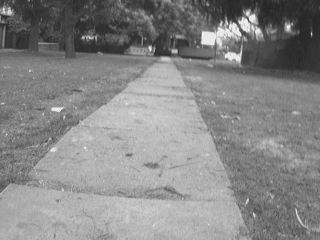
\includegraphics[scale=0.4]{deteccion_lineas/frame_1}};
  \draw[->] (0,0) coordinate(O) node[above left] {O}-- (5.5,0) coordinate(XE) node[above] {$x$};
    \draw[->] (0,0) -- (0,20) node[left] {$y$};
%  \draw[->] (5,0.2) coordinate(OPS)-- (5,5) coordinate(OPE) node[left] {$y'$};
  \draw[red] (-1,20) coordinate(l1_1)-- (3.5,-3) coordinate(l1_2) node[right] {$l_1$};
  %\draw[->] (O) coordinate(l1_1)-- (0.5,0) coordinate(l1_2) node[left] {$\rho_1$};
  \coordinate (l1c) at ($(l1_1)!(O)!(l1_2)$);
  \coordinate (l1x) at (intersection of O--XE and l1_1--l1_2);
  \draw [yellow,->] (O)--(l1c) node [midway, left] {$\vec{\rho}$} ;
\tkzMarkAngle[color=yellow,size=1cm,opacity=.4](l1c,O,l1x);
%\tkzLabelAngle[pos = (0.8,-5)](l1c,O,l1x){${\theta}$}
\node [yellow] (label) at (0.8,1.5){${\theta}$};
\tkzMarkRightAngle[color=yellow](O,l1c,l1x)
%\tkzMarkAngle[size=0.65,opacity=.4](l1c,l1x,O);


%  \coordinate (OP) at (intersection of O--XE and OPS--OPE);
%  \coordinate (l1cp) at ($(l1_1)!(OP)!(l1_2)$);
%  \draw [->] (OP)--(l1cp) node [midway, left] {${\rho_1}'$} ;
%\tkzMarkAngle[size=0.65cm,opacity=.4](l1cp,OP,XE);
%\tkzLabelAngle[pos = (-0.5,-0.5)](l1cp,OP,XE){${\theta_1}'$}
%\tkzMarkRightAngle(OP,l1cp,l1x);
 %  \fill[red] (l1x) circle (2pt);
  % \tkzLabelPoint[below](l1x){$x_1$};

\end{tikzpicture}
\end{center}
\caption{Transformadas de Hough, representación en coordenadas polares de las rectas}
\label{fig:hough}
\end{figure}

 Por último, de todas las rectas obtenidas por la transformada de Hough se seleccionan las 2 que mejor ajustan al modelo de camino recto. A continuación un pseudo-código del algoritmo que resume los pasos efectuados en cada iteración. 

\begin{algorithm}[H]
\caption{Detección de camino}
\label{alg:overview}
\begin{algorithmic}
\Procedure{porcesarVideo}{$video$}
	
    \While{ \CALL{FinDeVideo}{video} is $ $ false }
    	\State frame $\Leftarrow$ \CALL{proximoFrame}{video}
        \State \CALL{ecualizarHistograma}{frame}
        \State $[bordes,u_{min},u_{max},m\_gradiente,dir\_gradiente] \Leftarrow$ \CALL{Canny}{frame}
        \State $[lineas\_izq,lineas\_der] \Leftarrow$ \CALL{lineasHough}{bordes}
        \State $[idx\_izq,idx\_der] \Leftarrow$ \CALL{seleccionarBordesCamino}{lineas\_izq,lineas\_der,dir\_gradiente}
        \If{idx\_izq is not null and idx\_der is not null}
        	\State linea\_izq $\Leftarrow$ lineas\_izq$[$idx\_izq$]$
            \State linea\_der $\Leftarrow$ lineas\_der$[$idx\_der$]$
        	\State frame $\Leftarrow$ \CALL{drawLines}{frame,linea\_izq,linea\_izq}
        \EndIf
        \State \CALL{saveFrame}{frame}
    \EndWhile
\EndProcedure
\end{algorithmic}
\end{algorithm}


\section{Detalles de  Implementación}
\subsection{Ecualización de Histograma}

%A diferencia del algoritmo de detección de lineas de hough que se aplica independientemente al lado izquierdo y derecho de la imagen, la detección de bordes se aplica sobre toda la imagen. 
	La selección de un un umbral único que correctamente detecte ambos lados del camino puede ser difícil con condiciones de luz cambiantes y cuando no hay simetría con respecto al camino, es decir, con un camino que en un lado limita, por ejemplo,  con césped y en el otro lado limita con otro tipo de material, generando módulos de gradientes diferentes para cada borde del camino. La selección de un umbral muy alto nos puede hacer perder uno de los bordes del camino y uno muy bajo introduce falsos bordes complicando la selección de lineas con hough. \\ 
	A fin de lograr robustez a las variaciones de luz y facilitar detección en ocasiones como la descrita anteriormente se hace una  ecualización de histograma antes de detectar los bordes.
    Obviamente la ecualización de histograma aumenta el contraste en toda la imagen, haciendo que aparezcan "falsos" bordes, por lo que es necesario hacer un suavizado de la imagen como parte de la detección de bordes. 
    En la figura ~\ref{fig:ecualizacion} se puede observar 
   observar los bordes y lineas detectadas para un frame sin ecualizar, uno ecualizado sin suavizado y uno con ecualización y suavizado. Si se compara las lineas detectadas entre el frame sin y con suavizado, figuras ~\ref{fig:ecualizacion/umbral_unificado_con_eq_sin_suav_lineas} y ~\ref{fig:ecualizacion/umbral_unificado_con_eq_lineas} , no se nota mucha diferencia y esto se debe a ciertas restricciones en los ángulos de las rectas posibles que se  implementa en la transformada de hough. 
    
\begin{figure}[H]
\myss{0.5}{ecualizacion/umbral_unificado_sin_eq_borders}{Bordes frame sin ecaulizar}
\myss{0.5}{ecualizacion/umbral_unificado_sin_eq_lineas}{Lineas frame sin ecaulizar}
\myss{0.5}{ecualizacion/umbral_unificado_con_eq_sin_suav_borders}{Bordes frame ecualizado, sin suavizado}
\myss{0.5}{ecualizacion/umbral_unificado_con_eq_sin_suav_lineas}{Lineas frame ecualizado, sin suavizado}
\myss{0.5}{ecualizacion/umbral_unificado_con_eq_borders}{Bordes frame ecualizado y suavizado}
\myss{0.5}{ecualizacion/umbral_unificado_con_eq_lineas}{Lineas frame ecualizado y suavizado}
\caption{Efectos de ecualización de histograma}
\label{fig:ecualizacion}
\end{figure}

\subsection{Detección de bordes} \label{sec:bordes}

Para la detección de bordes se utiliza el algoritmo de canny modificado para utilizar solo una de las direcciones del gradiente a fin minimizar la detección de lineas horizontales que no son de nuestro interés y ademas considerarlas tiene impacto en la cantidad de cómputos necesarios al aplicar hough. En la figura ~\ref{fig:bordes} se muestra los diferentes resultados obtenidos al utilizar modulo de gradiente y gradiente en una dirección.


\begin{figure}[H]
\myss{0.5}{bordes/bordes_modulo_gradiente_bordes}{Bordes detectados usando modulo gradiente}
\myss{0.5}{bordes/bordes_modulo_gradiente_lineas}{Lineas detectadas a partir de bordes en figura ~\ref{fig:bordes/bordes_modulo_gradiente_bordes}}
\myss{0.5}{bordes/bordes_derivada_direccion_x_bordes}{Bordes detectados usando modulo gradiente}
\myss{0.5}{bordes/bordes_derivada_direccion_x_lineas}{Lineas detectadas a partir de bordes en figura ~\ref{fig:bordes/bordes_derivada_direccion_x_bordes}}
\caption{Bordes utilizando modulo e gradiente y derivada en una única dirección}
\label{fig:bordes}
\end{figure}

La selección del umbral se realiza en función de la media del modulo de la derivada parcial en x. Se experimento con múltiples valores y  los mejores resultados se obtuvieron con $u_{min} = 2 \mu$ y $ u_{max} = \frac{3}{2} u_{min}$

\subsection{Transformada de Hough} \label{sec:hough}

	En las primeras versiones del algoritmo se aplicaba hough  y se buscaban ambos bordes del camino al mismo tiempo. El algoritmo seleccionaba todas las rectas que tuviesen mas votos que $0.9 \cdot max\_votos$, donde max\_votos son los votos recibidos por la recta más votada. Este enfoque solo funcionaba bien en frames donde ambos bordes tenían longitudes similares. En casos como los que se muestran en la figura ~\ref{fig:corridas} para que el borde mas corto fuese seleccionado era necesario bajar el umbral a valores que aumentaban considerablemente el número de lineas encontradas, aumentando la cantidad de procesamiento necesario y dificultando el proceso de selección de los bordes. \\
\begin{figure}[H]
\begin{center}
\myss{0.4}{deteccion_lineas/frame_117}{}
\myss{0.4}{deteccion_lineas/frame_137}{}
\caption{Bordes de camino de longitudes diferentes}
\label{fig:corridas}
\end{center}
\end{figure}
Para resolver el problema se modificó el algoritmo para que  trabajara con 2 umbrales en simultaneo y considerando solo una porción de la matriz acumuladora de votos. Primero se busca el borde izquierdo, las lineas con más votos con $\rho > 0 $  y $ 0 \leq \theta \leq \frac{\pi}{2} $. Luego se busca el borde derecho, lineas con $\theta$ entre $ \frac{\pi}{2} \leq \theta \leq \pi  $. Esto mejoro la selección de lineas en la mayoría de los casos, pero el echo de tener umbral relativamente bajo hacía aparecer rectas horizontales por acumulación de votos de bordes pequeños a lo ancho de la imagen o imperfecciones en el camino. \\
	Para lograr una detección de bordes mas robusta se decidió dividir la imagen en lado izquierdo y derecho, generando una matriz de votos independiente para cada sección,esto permitió reducir el impacto de pequeños bordes considerablemente. Se mantienen las restricciones de $\rho$ y $\theta$  introducidas en la versión anterior.\\
Los valores obtenidos al aplicar hough al lado derecho de la imagen están desplazados y es necesarios convertir las coordenadas al sistema original, ver figuras ~\ref{fig:rho_positivo} y ~\ref{fig:rho_negativo} .Las ecuaciones para las rectas con $\rho$ positivo y negativos, $l_1$  y $l_2$ respectivamente, están dadas por:
\begin{align*}
\rho_{1}' = x' cos(\theta_{1}) + y' sen(\theta_{1})\\
\rho_{2}' = x' cos(\theta_{2}) + y' sen(\theta_{2})
\end{align*}
La intersección de $l_1$  y $l_2$ con el eje x en $x_1$ y $x_2$ se puede calcular de las siguiente forma:
\begin{align*}
x_1 = \frac{\rho'}{cos(\theta_{1}')}\\
x_2 = \frac{\rho'}{cos(\theta_{2}')} 
\end{align*}
  Siendo $N_2$ las distancia entre el eje $O$ e $O'$, se puede calcular los  $\rho$ del sistema de coordenadas original con la siguiente ecuación:
\begin{align*}
\rho_1  = x_1 cos(\pi - \theta_{1}')=\left(N_2 - \left| \frac{\rho_{1}'}{cos(\pi - \theta_{1}')}\right|\right) cos(\pi - \theta_{1}')  = N_2 cos(\pi - \theta_{1}') - \rho_{1}'\\
\rho_2 = ( x_2 + N_2 )  cos(\theta{2}')=\left(\left|\frac{\rho_{2}'}{cos(\pi-\theta_{2}')}\right|+N_2\right) cos(\pi - \theta_{2}') = N_2 cos(\pi - \theta_{2}') + \rho_{2}'
\end{align*}
En el tercer termino se puede sacar el modulo dado que $\theta_{1}$ y $\theta_{2}$ son mayores que $ \frac{\pi}{2}$ por lo que el angulo evaluado en por el coseno siempre va a estar entre 0 y $ \frac{\pi}{2}$, generando un resultado positivo. Luego se puede calcular $\rho$ en el sistema original para cualquier signo de $\rho'$ con la siguiente ecuación:
\begin{align*}
\rho = N_2 cos(\pi - \theta') - \rho'
\end{align*}

\begin{figure}[H]


\begin{tikzpicture}[y=-1cm]
  \draw[->] (0,2) coordinate(O) node[below left] {O}-- (10,2) coordinate(XE) node[below] {$x$};
  \draw[->] (0,0.2) -- (0,5) node[left] {$y$};
  \draw[->] (5,0.2) coordinate(OPS)-- (5,5) coordinate(OPE) node[left] {$y'$};
  \draw[red] (6,5) coordinate(l1_1)-- (0.5,0) coordinate(l1_2) node[right] {$l_1$};
  %\draw[->] (O) coordinate(l1_1)-- (0.5,0) coordinate(l1_2) node[left] {$\rho_1$};
  \coordinate (l1c) at ($(l1_1)!(O)!(l1_2)$);
  \coordinate (l1x) at (intersection of O--XE and l1_1--l1_2);
  \draw [->] (O)--(l1c) node [midway, left] {${\vec{\rho}}$} ;
\tkzMarkAngle[size=0.8cm,opacity=.4](l1x,O,l1c);
%\tkzLabelAngle[pos = (0.4,10)](l1c,O,l1x){${\theta}$}
\tkzMarkRightAngle(O,l1c,l1x)
\tkzMarkAngle[size=0.65cm,opacity=.4](l1c,l1x,O);


  \coordinate (OP) at (intersection of O--XE and OPS--OPE);
  \coordinate (l1cp) at ($(l1_1)!(OP)!(l1_2)$);
  \draw [->] (OP)--(l1cp) node [midway, left] {$\vec{{\rho_1}'}$} ;
\tkzMarkAngle[size=0.65cm,opacity=.4](l1cp,OP,XE);
%\tkzLabelAngle[pos = (-0.3,-1)](l1cp,OP,XE){${\theta_1}'$}
\tkzMarkRightAngle(OP,l1cp,l1x);
   \fill[red] (l1x) circle (2pt);
   \tkzLabelPoint[below](l1x){$x_1$};
	\tkzLabelPoint[below right](OP){${\theta_1}'$};
   \tkzLabelPoint[above right](0.25,1.95){${\theta}$};
\end{tikzpicture}

\caption{Transformación de coordenadas con $\rho > 0 $}
\label{fig:rho_positivo}
\end{figure}

\begin{figure}[H]

\begin{tikzpicture}[y=-1cm]
  \draw[->] (-2,2)  -- (10,2) coordinate(XE) node[below] {$x$};
  \draw[->] (0,0.2) -- (0,5) node[left] {$y$};
  \draw[->] (5,0.2) coordinate(OPS)-- (5,5) coordinate(OPE) node[left] {$y'$};
  \draw[red] (9,5) coordinate(l1_1)-- (5.5,-2) coordinate(l1_2) node[right] {$l_2$};

  %\draw[->] (O) coordinate(l1_1)-- (0.5,0) coordinate(l1_2) node[left] {$\rho_1$};
  \coordinate (O) at (0,2);
  \coordinate (NE) at (-2,2);
  \coordinate (l1c) at ($(l1_1)!(O)!(l1_2)$);
  \coordinate (l1x) at (intersection of O--XE and l1_1--l1_2);
  \draw [->] (O)--(l1c) node [midway, left] {$\vec{{\rho}}$} ;
\tkzMarkAngle[size=1cm,opacity=.4](l1c,O,NE);
%\tkzLabelAngle[pos = (0.5,0.5)](l1c,O,l1x){${\theta}$}
\tkzLabelPoint[above](-0.5,2){$\theta$};
\tkzMarkRightAngle(O,l1c,l1x)
%\tkzMarkAngle[size=0.65cm,opacity=.4](l1c,l1x,O);
%\tkzLabelAngle[pos=(-0.5,-0.5)](l1c,l1x,O){${\beta}$}

  \coordinate (OP) at (intersection of O--XE and OPS--OPE);
  \coordinate (l1cp) at ($(l1_1)!(OP)!(l1_2)$);
  \draw [->] (OP)--(l1cp) node [midway, right] {$\vec{{\rho_2}'}$} ;
\tkzMarkAngle[size=1cm,opacity=.4](l1cp,OP,O);
%\tkzLabelAngle[pos =1](l1cp,OP,XE){${\theta'}$}
\tkzMarkRightAngle(OP,l1cp,l1x);
   \fill[red] (l1x) circle (2pt);
      \tkzLabelPoint[below](l1x){$x_2$};
\tkzLabelPoint[above left](4.9,2){$\theta_{2}'$};

\end{tikzpicture}
\caption{Transformación de coordenadas para rectas con $\rho < 0 $}
\label{fig:rho_negativo}
\end{figure}



\subsection{Selección de lineas}

	La detección de lineas mediante la transformada de hough puede devolver mas de 1 recta por borde de camino. A fin de seleccionar las lineas que mejor ajustan al modelo de  camino recto, se utiliza la propiedad de que ambos bordes del camino van a tener dirección de gradiente opuestas. 
	Para cada par de bordes izquierdos y derechos se calcula la intersección  de las lineas y se suman las direcciones del gradiente punto a punto, seleccionando las rectas que minimizan la suma. Se consideran los puntos desde la intersección(punto de fuga) hasta el mayor y de la recta mas corta.\\
    
\begin{algorithm}[H]
\caption{Selector de bordes de camino}
\label{alg:selector}
\begin{algorithmic}
\Procedure{seleccionarBordesCamino}{lineas\_izq,lineas\_der,dir\_gradiente}


	\State suma\_min $ \Leftarrow \inf$
    \State linea\_izq $ \Leftarrow $ \Null
    \State linea\_der $ \Leftarrow $ \Null
    %\For{k}
    %
    	\ForAll{lz \IN$ $ lineas\_izq}
        	    \ForAll{ld \IN$ $ lineas\_der}
        			\State $[x,y] \Leftarrow $ \CALL{calcularInterseccion}{lz,ld}
                    \State dir\_izq $\Leftarrow$ \CALL{obtenerAngulosGradienteEnLinea}{lz}
                    \State dir\_der $\Leftarrow$ \CALL{obtenerAngulosGradienteEnLinea}{ld}
                    \State max\_y $ \Leftarrow $ \CALL{max}{$largo(dir\_izq),largo(dir\_der)$}
                    \State tsum = 0
                    \For{ i $ $\FROM$ $\CALL{max}{1,y} \UNTIL$ $max\_y}
                    	\State tsum $+= \Leftarrow |dir\_izq(i) + dir\_der(i)|$  
                    \EndFor
                    \If{$tsum < min\_sum$}
                        \State linea\_izq $ \Leftarrow $ lz
                        \State linea\_der $ \Leftarrow $ ld                   
                    \EndIf               
            \EndFor
        \EndFor
    %\EndFor
     \State \Return $[linea\_izq,linea\_der]$
\EndProcedure
\end{algorithmic}
\end{algorithm}


    Este procedimiento demostró ser útil solo cuando las rectas devueltas por hough están "cercanas" a los bordes del camino. Es decir la transformada hough devuelve una recta horizontal o con $\theta$ cercano a $\frac{pi}{2}$, el echo de que menos puntos participen de la suma hace que el selector tienda a seleccionar dichas rectas. 


\section{Conclusión}

El algoritmo desarrollado logro detectar satisfactoriamente el borde en los 2 caminos con los que se expermineto, aunque el buen funcionamiento del algoritmo depende fuertemente de la extracción de lineas efectuada con la transformada de hough.Un mal resultado de la transformada de hough,por lo general, no puede ser recuperado por selector de bordes. 


\subsection{Bibliografia}

\begin{thebibliography}{}
                \bibitem{lib:jain}
                        Anil K. Jain,
                        \textit{Fundamentals of Digital Image Processing},
                        Prentice Hall. 
                \bibitem{lib:gonzalez}
                        Rafael C.Gonzalez. Richard E.Woods,
                        \textit{Digital Image Processing},
                        Addison-Wesley. 3ra. Edición. 
                \bibitem{lib:ieee}
                       Hunjae Yoo, Ukil Yang, and Kwanghoon Sohn,
                        \textit{Gradient-Enhancing Conversion for Illumination-Robust Lane Detection},
                        IEEE TRANSACTIONS ON INTELLIGENT TRANSPORTATION SYSTEMS, VOL. 14, NO. 3, SEPTEMBER 2013 
                \bibitem{lib:real}
                        Abdulhakam.AM.Assidiq, Othman O. Khalifa, Md. Rafiqul Islam, Sheroz Khan,
                        \textit{Real Time Lane Detection for Autonomous Vehicles},
                        Proceedings of the International Conference on Computer and Communication Engineering 2008 
                \bibitem{lib:web1}
                        \textit{http://matlabtricks.com/post-41/understanding-the-hough-transform-2}
                \bibitem{lib:web2}
                        \textit{http://homepages.inf.ed.ac.uk/rbf/HIPR2/hough.htm}
\end{thebibliography}
\end{document}
